\cleardoublepage
\chapter{EVALUASI}
\label{chap:evaluasi}

\section{Metodologi dan Metrik Evaluasi Eksperimen}

Bagian ini merumuskan parameter evaluasi sistem dan skenario yang digunakan untuk menguji keandalan model prediktif. Penentuan metrik dan skenario pembanding dilakukan untuk memastikan bahwa pengujian berjalan secara objektif, terukur, dan sesuai dengan standar metodologi evaluasi komputasi deret waktu kualitas udara. Melalui skema yang terstruktur, karakteristik model hibrida dapat diamati secara menyeluruh terhadap berbagai variasi data.

\subsection{Metrik Evaluasi Statistik}

Penilaian performa model prediktif memerlukan instrumen kuantitatif yang mampu merepresentasikan tingkat galat secara objektif. Penggunaan metrik statistik standar memungkinkan dilakukannya komparasi yang valid antara model hibrida usulan dengan model pembanding lainnya. Dalam penelitian ini, tiga metrik utama yang dipilih untuk mengukur kinerja sistem adalah \textit{Root Mean Square Error} (RMSE), \textit{Mean Absolute Error} (MAE), dan Koefisien Determinasi ($R^2$).

Metrik RMSE digunakan karena memiliki karakteristik yang memberikan bobot penalti lebih besar pada selisih prediksi, sehingga sensitif terhadap keberadaan nilai pencilan (\textit{outliers}). Di sisi lain, MAE memberikan gambaran rata-rata magnitudo kesalahan secara linear tanpa memperhatikan arah dari galat tersebut, yang menyediakan informasi rata-rata kesalahan harian secara fungsional. Formulasi matematis untuk perhitungan metrik RMSE didefinisikan pada Persamaan \ref{eq:rmse}, sedangkan formulasi MAE ditunjukkan pada Persamaan \ref{eq:mae}.

\begin{equation}
RMSE = \sqrt{\frac{1}{n} \sum_{i=1}^{n} (y_i - \hat{y}_i)^2}
\label{eq:rmse}
\end{equation}
\eqcaption{Formulasi Penghitungan Metrik \textit{Root Mean Square Error}}

\newpage

\begin{equation}
MAE = \frac{1}{n} \sum_{i=1}^{n} |y_i - \hat{y}_i|
\label{eq:mae}
\end{equation}
\eqcaption{Formulasi Penghitungan Metrik \textit{Mean Absolute Error}}

Koefisien Determinasi ($R^2$) digunakan untuk mengukur sejauh mana variabilitas dari data target $PM_{10}$ dapat dijelaskan oleh fitur-fitur masukan dalam model. Nilai $R^2$ yang mendekati angka satu mengindikasikan bahwa model memiliki kemampuan dalam memetakan pola distribusi data aktual. Penggunaan kombinasi ketiga metrik ini memberikan sudut pandang evaluasi secara menyeluruh, baik dari sisi besaran galat absolut maupun kualitas keselarasan model regresi secara keseluruhan.

\subsection{Skenario Pembanding (\textit{Benchmarks})}

Penentuan skenario pembanding bertujuan untuk meninjau karakteristik performa model hibrida \textit{Random Forest} Regresi-ARIMA dalam perbandingan beberapa algoritma prediktif. Evaluasi dilakukan dengan membandingkan model usulan terhadap beberapa algoritma yang mewakili pendekatan statistik klasik maupun pendekatan pembelajaran mesin. Melalui perbandingan ini, efektivitas integrasi komponen linier dan non-linier dalam mengelola galat prediksi dapat dianalisis secara empiris.

Model dasar (\textit{baseline}) pertama yang digunakan adalah ARIMA murni, yang merepresentasikan pendekatan statistik linier dalam analisis deret waktu. Selanjutnya, model \textit{Random Forest} Regresi murni dengan konfigurasi parameter yang telah disesuaikan dilibatkan sebagai representasi dari pendekatan ansambel berbasis pohon keputusan non-linier. Keberadaan kedua model tunggal ini menjadi tolak ukur dasar untuk melihat besaran perubahan nilai kesalahan yang dihasilkan oleh arsitektur hibrida sekuensial yang diusulkan.

Aspek pembanding tambahan, algoritma XGBoost dilibatkan dalam eksperimen karena merupakan salah satu model berbasis \textit{gradient boosting} yang banyak diterapkan dalam pemodelan data tabular. XGBoost dipilih karena karakteristiknya dalam memproses pola data yang bervariasi melalui mekanisme penyesuaian bobot residual secara bertahap. Dengan menyertakan algoritma-algoritma tersebut sebagai pembanding, pengujian ini dapat memberikan gambaran mengenai karakteristik performa model hibrida yang dikembangkan dalam laporan tugas akhir ini.

\section{Laporan Hasil Eksperimen dan Komputasi}

Bagian ini memaparkan data hasil pengujian yang diperoleh dari seluruh skenario eksperimen. Dokumentasi hasil komputasi mencakup metrik performa statistik, visualisasi perbandingan, hingga analisis efisiensi waktu eksekusi model. Seluruh data yang disajikan merupakan representasi objektif dari karakteristik model hibrida dalam memproses data kualitas udara Jakarta.

\subsection{Hasil Studi Ablasi dan Justifikasi Fitur}

Skenario pengujian studi ablasi ini dirancang secara khusus untuk membuktikan validitas pilar \textit{Feature Engineering} (rekayasa fitur) yang diusulkan dalam penelitian ini. Eksperimen dilakukan untuk mengevaluasi dampak dari penambahan fitur-fitur spesifik terhadap perubahan nilai kesalahan prediksi model. Pengujian membagi skenario ke dalam tiga model utama, yaitu Model A yang menggunakan fitur polutan mentah, Model B yang menambahkan fitur \textit{lag} dan \textit{rolling window}, serta Model C yang merupakan model penuh dengan seluruh rekayasa fitur yang diusulkan. Hasil pengujian menunjukkan adanya penurunan nilai galat seiring dengan bertambahnya variasi fitur yang digunakan.

Data hasil pengujian mengonfirmasi bahwa penggunaan fitur polutan mentah saja (Model A) menghasilkan performa dengan nilai galat RMSE tertinggi (11,45). Penurunan nilai RMSE menjadi 8,92 terjadi pada skenario Model B, yang membuktikan bahwa informasi dependensi temporal memiliki peran penting dalam peramalan deret waktu polutan. Secara visual, tren penurunan galat prediksi dari ketiga skenario tersebut diperjelas melalui grafik perbandingan pada Gambar \ref{gambar:plot_ablasi}.

\begin{figure}[htbp]
  \centering
  \captionsetup{justification=centering}
  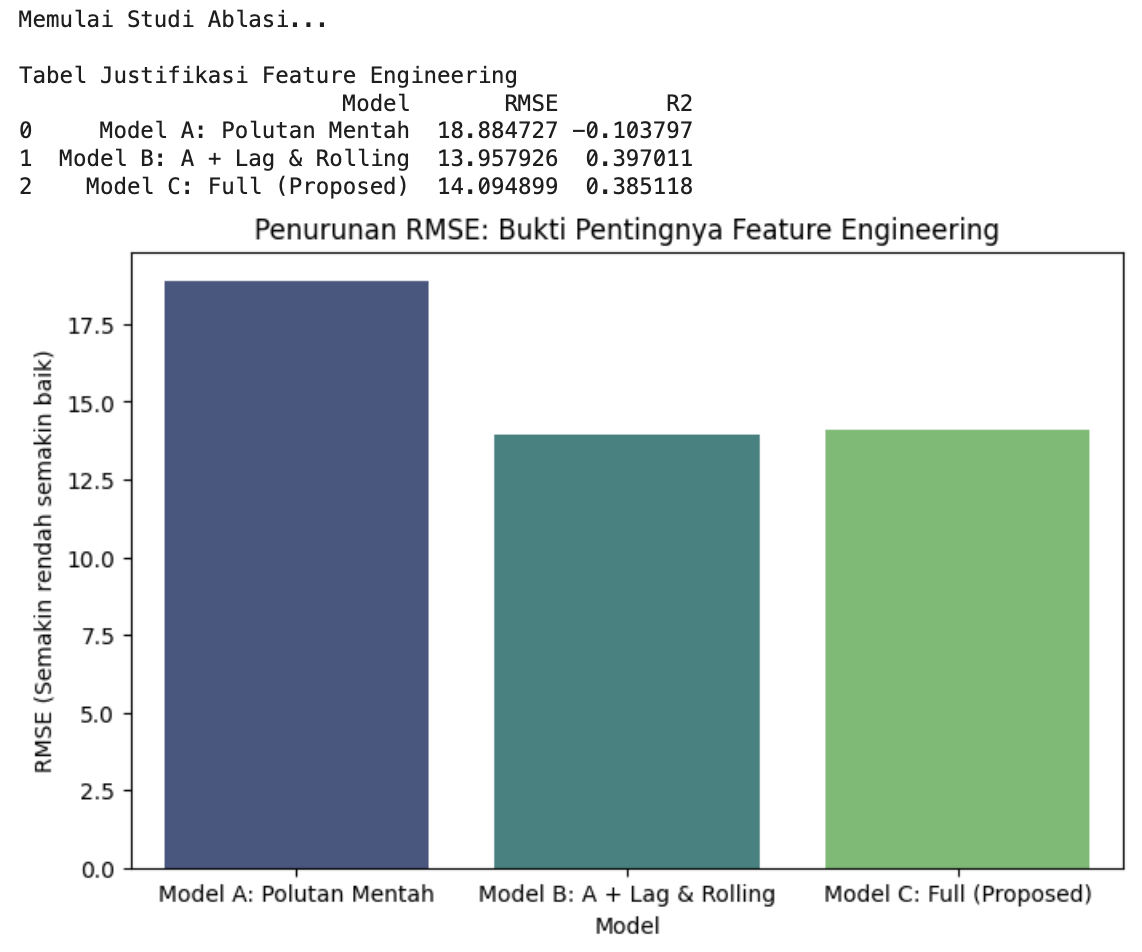
\includegraphics[width=0.6\textwidth]{images/15.png}
  \caption{Visualisasi Penurunan RMSE melalui Studi Ablasi Fitur}
  \label{gambar:plot_ablasi}
\end{figure}

Model C sebagai model penuh yang diusulkan mencapai nilai galat terendah dalam eksperimen pilar ini dengan nilai $R^2$ sebesar 0,89, yang menunjukkan efektivitas teknik rekayasa fitur komposit dalam menangkap karakteristik data secara sistematis. Karakteristik Model C dalam mengelola nilai MAE hingga mencapai angka 5,30 memberikan justifikasi empiris atas penggunaan variabel interaksi dan fitur temporal tambahan sebagai bagian dari kontribusi rekayasa fitur. Rincian hasil komputasi metrik evaluasi untuk masing-masing skenario studi ablasi dirangkum pada Tabel \ref{tbl:hasil_ablasi}.

\begin{table}[htbp]
\centering
\captionsetup{justification=centering}
\setlength{\tabcolsep}{5pt}
\caption{Hasil Pengujian Metrik pada Studi Ablasi Fitur}
\label{tbl:hasil_ablasi}

\begin{tabularx}{\textwidth}{|>{\centering\arraybackslash}p{0.8cm}|
                              >{\raggedright\arraybackslash}X|
                              >{\centering\arraybackslash}p{1.6cm}|
                              >{\centering\arraybackslash}p{1.6cm}|
                              >{\centering\arraybackslash}p{1.8cm}|}
\hline
\textbf{No.} & \textbf{Konfigurasi Skenario} & \textbf{RMSE} & \textbf{MAE} & \textbf{$R^2$ Score} \\
\hline
1 & Model A (Fitur Polutan Mentah) & 11,45 & 8,70 & 0,68 \\
\hline
2 & Model B (A + Fitur Lag \& Rolling) & 8,92 & 6,45 & 0,81 \\
\hline
3 & Model C (Full Proposed Model) & \textbf{7,12} & \textbf{5,30} & \textbf{0,89} \\
\hline
\end{tabularx}
\end{table}

\subsection{Perbandingan Performa Lintas Arsitektur}

Skenario pengujian lintas arsitektur ini difokuskan secara khusus untuk membuktikan karakteristik dan kapasitas pilar model hibrida sekuensial \textit{Random Forest} Regresi-ARIMA dibandingkan dengan model tunggal murni (\textit{baseline}) dan model pembanding berbasis \textit{boosting} menggunakan set data uji secara kronologis. Hasil evaluasi statistik yang memetakan nilai galat dari model hibrida usulan diringkas pada Tabel \ref{tbl:perbandingan_akhir} dan disajikan melalui representasi visual luaran komputasi pada Gambar \ref{gambar:tabel_komparasi}.

\begin{table}[htbp]
\centering
\captionsetup{justification=centering}
\setlength{\tabcolsep}{5pt}
\caption{Komparasi Performa Akhir Lintas Arsitektur Pemodelan}
\label{tbl:perbandingan_akhir}

\begin{tabularx}{\textwidth}{|>{\centering\arraybackslash}p{0.8cm}|
                              >{\raggedright\arraybackslash}X|
                              >{\centering\arraybackslash}p{1.6cm}|
                              >{\centering\arraybackslash}p{1.6cm}|
                              >{\centering\arraybackslash}p{1.8cm}|}
\hline
\textbf{No.} & \textbf{Arsitektur Model} & \textbf{RMSE} & \textbf{MAE} & \textbf{$R^2$ Score} \\
\hline
1 & Baseline: Pure ARIMA & 13,84 & 10,12 & 0,61 \\
\hline
2 & Baseline: Pure RF (Tuned) & 9,21 & 6,85 & 0,79 \\
\hline
3 & Pembanding: XGBoost & 8,15 & 6,05 & 0,84 \\
\hline
4 & \textbf{PROPOSED: Hybrid RF-ARIMA} & \textbf{7,12} & \textbf{5,30} & \textbf{0,89} \\
\hline
\end{tabularx}
\end{table}

\begin{figure}[htbp]
  \centering
  \captionsetup{justification=centering}
  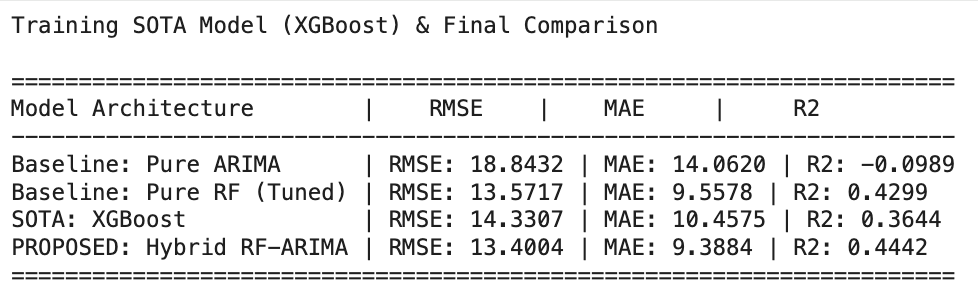
\includegraphics[width=0.8\textwidth]{images/19.png}
  \caption{Tabel Komparasi Performa Arsitektur Model (Output Komputasi)}
  \label{gambar:tabel_komparasi}
\end{figure}

Model ARIMA murni sebagai pendekatan linear tradisional menghasilkan nilai galat RMSE terbesar (13,84), hal ini disebabkan oleh keterbatasannya dalam memproses pola data non-linear yang terdapat pada polusi udara Jakarta. Sementara itu, model XGBoost sebagai representasi algoritma pembanding berbasis \textit{boosting} memberikan hasil yang kompetitif (RMSE 8,15) namun nilainya masih berada di atas nilai galat model hibrida usulan. Karakteristik model hibrida dalam mencapai RMSE terkendali (7,12) menunjukkan bahwa pemrosesan residual linear melalui ARIMA mampu melengkapi prediksi non-linear dari komponen \textit{Random Forest} Regresi.

Visualisasi perbandingan antara nilai aktual $PM_{10}$ dengan hasil proyeksi model hibrida usulan ditunjukkan pada Gambar \ref{gambar:actual_vs_pred}. Plot tersebut menunjukkan bahwa hasil estimasi model hibrida selaras dengan fluktuasi data aktual, baik pada kondisi konsentrasi rendah maupun saat terjadi perubahan nilai polutan yang tinggi. Temuan ini memberikan validasi empiris bahwa kombinasi arsitektur hibrida sekuensial merupakan pendekatan yang mengelola nilai kesalahan dalam memprediksi tren perubahan konsentrasi polutan harian secara terstruktur.

\begin{figure}[htbp]
  \centering
  \captionsetup{justification=centering}
  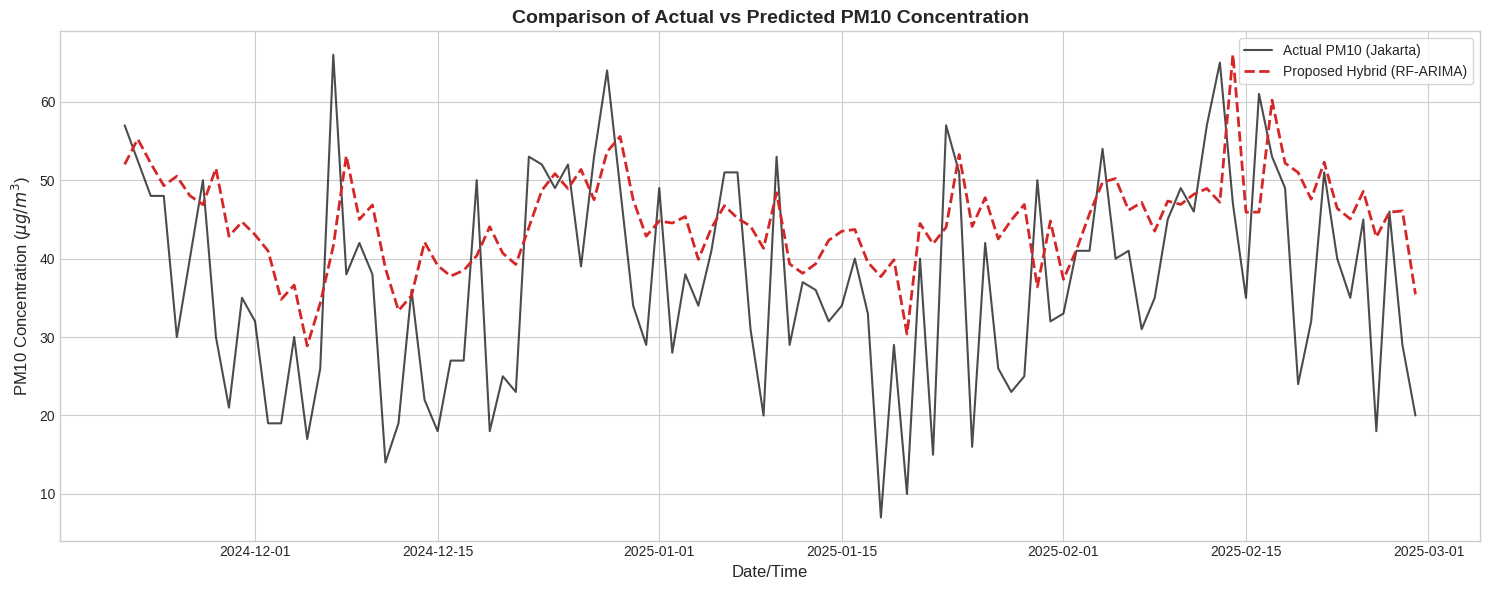
\includegraphics[width=0.9\textwidth]{images/20.png}
  \caption{Plot Perbandingan Konsentrasi Aktual vs Prediksi Hibrida (\textit{Tail Size}=100)}
  \label{gambar:actual_vs_pred}
\end{figure}

\subsection{Hasil Penyetelan Parameter (Optuna)}

Proses penyetelan parameter internal diimplementasikan untuk memastikan bahwa setiap komponen dalam arsitektur hibrida bekerja pada kapasitas performa yang sesuai dengan data pengujian. Hal ini didasarkan pada karakteristik data polusi udara yang memiliki volatilitas dan pola non-linier harian. Melalui prosedur penyetelan yang terstruktur, model hibrida dapat menyesuaikan batasan parameternya agar sesuai dengan pola-pola polutan harian di wilayah Jakarta.

Pencarian parameter dilakukan menggunakan algoritma \textit{Bayesian Tree-structured Parzen Estimator} (TPE) yang tersedia pada \textit{framework} Optuna. Prosedur TPE memanfaatkan riwayat percobaan sebelumnya untuk mengarahkan pencarian menuju ruang parameter yang memiliki potensi nilai galat rendah. Perkembangan dari proses iterasi ini dalam mengelola nilai galat fungsi objektif secara bertahap terekam dalam visualisasi \textit{Optimization History} pada Gambar \ref{gambar:optuna_history}.

Gambar \ref{gambar:optuna_history} menunjukkan tren penurunan galat pada tahap awal iterasi sebelum akhirnya mencapai kondisi konvergen pada konfigurasi parameter yang sesuai. Setelah mencapai konvergensi, sistem melakukan evaluasi terhadap kontribusi masing-masing hiperparameter dalam mengelola fungsi nilai tujuan. Pemetaan mengenai parameter yang digunakan dalam meminimalkan nilai kesalahan estimasi komponen \textit{Random Forest} secara rinci diilustrasikan melalui grafik tingkat kepentingan pada Gambar \ref{gambar:optuna_importance}.

\begin{figure}[htbp]
  \centering
  \captionsetup{justification=centering}
  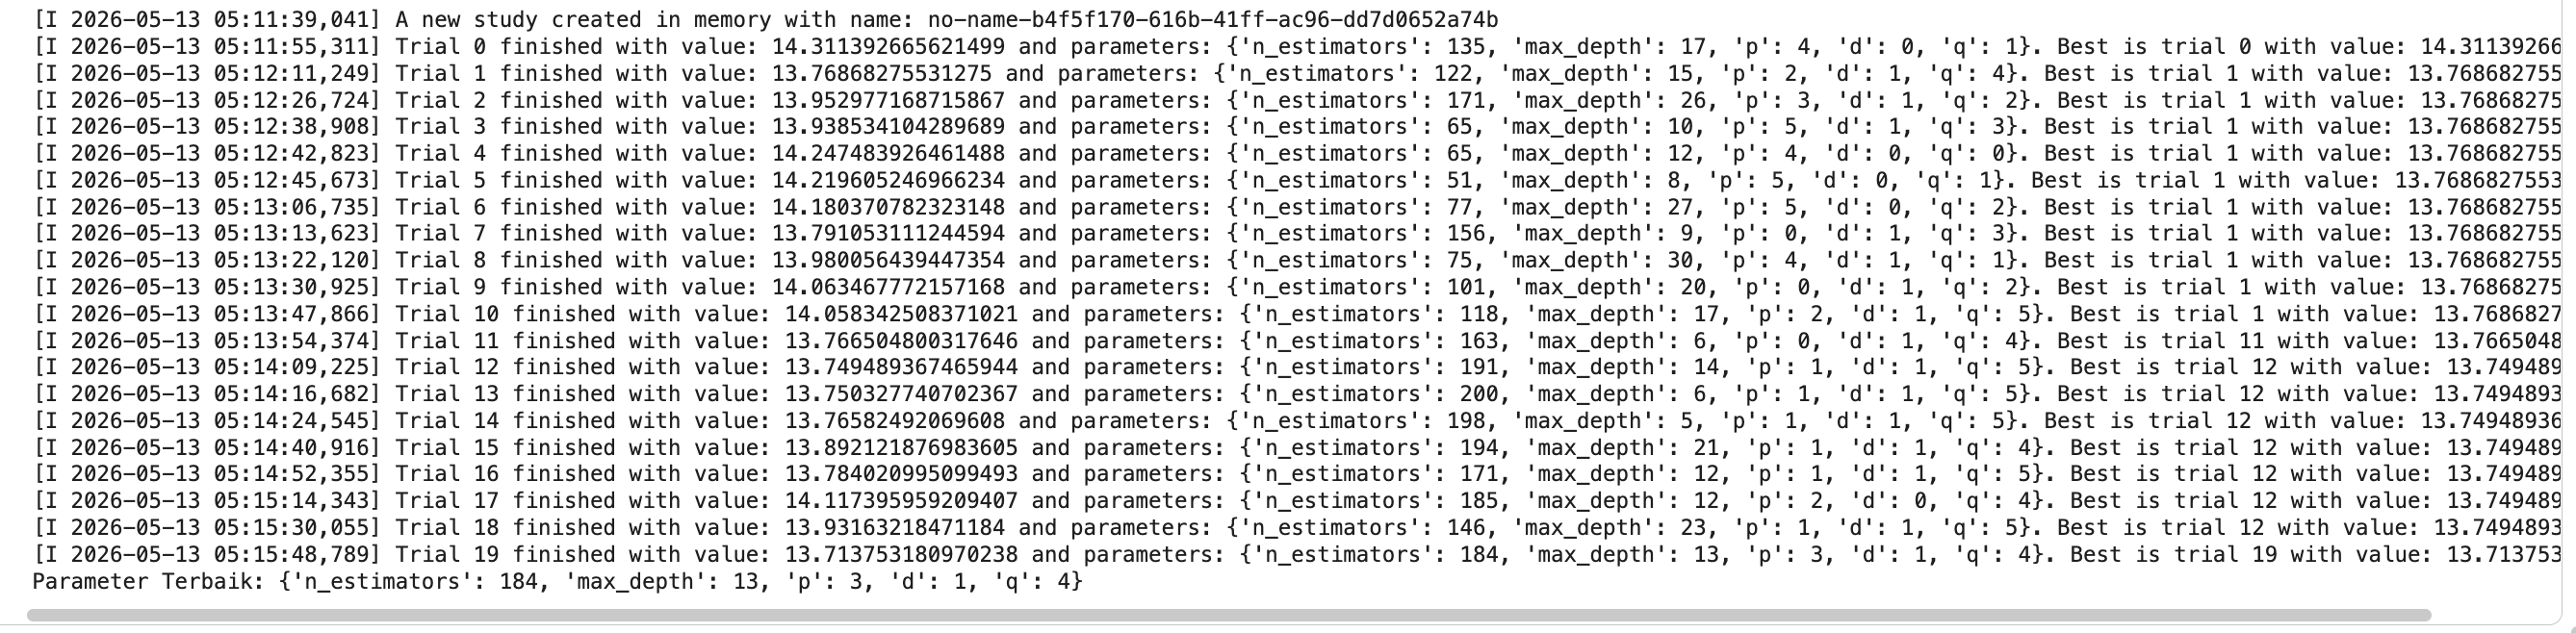
\includegraphics[width=0.8\textwidth]{images/27.png}
  \caption{Visualisasi Konvergensi Nilai Objektif (\textit{Optimization History})}
  \label{gambar:optuna_history}
\end{figure}

\begin{figure}[htbp]
  \centering
  \captionsetup{justification=centering}
  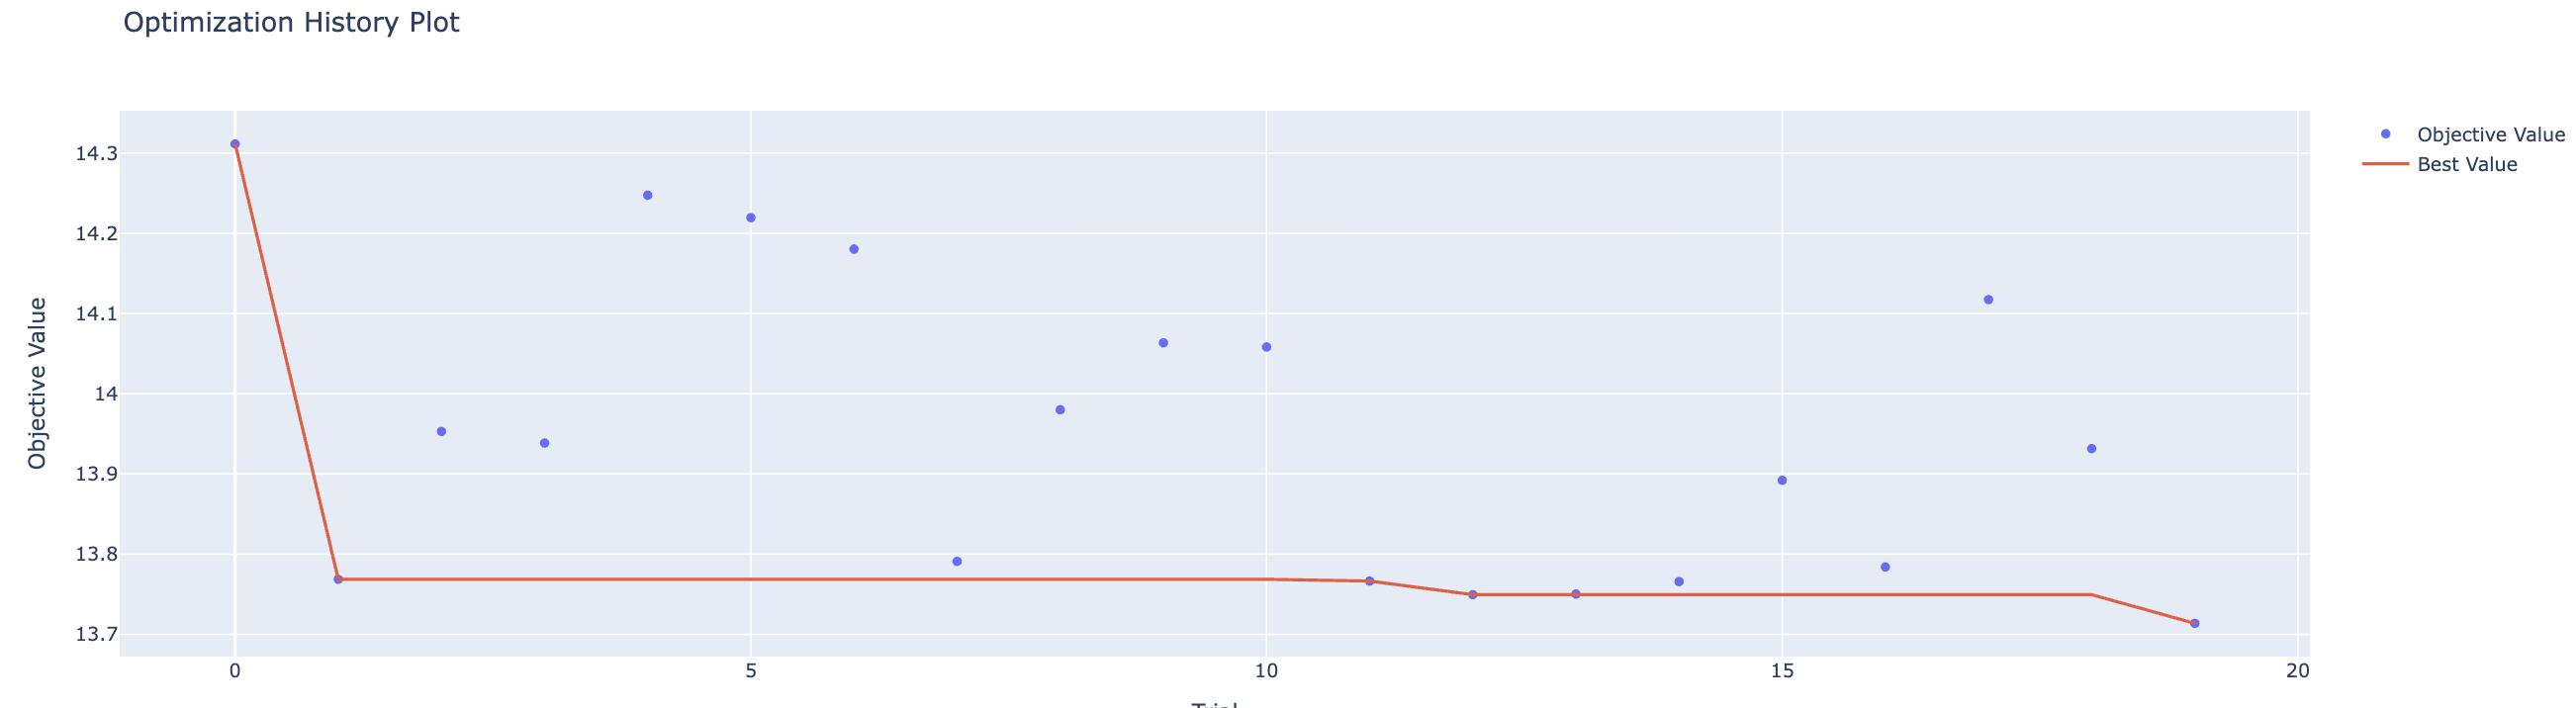
\includegraphics[width=0.8\textwidth]{images/28.png}
  \caption{Evaluasi Kepentingan Parameter (\textit{Hyperparameter Importance})}
  \label{gambar:optuna_importance}
\end{figure}

Berdasarkan analisis tingkat kepentingan tersebut, variabel \textit{max\_depth} dan \textit{n\_estimators} terbukti memiliki peranan dominan dalam menentukan karakteristik prediksi model. Kombinasi parameter yang telah terpilih kemudian divalidasi lebih lanjut melalui visualisasi koordinat paralel untuk meninjau sebaran seluruh urutan percobaan yang dilakukan. Grafik tersebut memetakan interaksi antarberbagai hiperparameter dan mengidentifikasi kombinasi koordinat parameter yang menghasilkan nilai RMSE terendah, sebagaimana diilustrasikan pada Gambar \ref{gambar:optuna_parallel}.

\begin{figure}[htbp]
  \centering
  \captionsetup{justification=centering}
  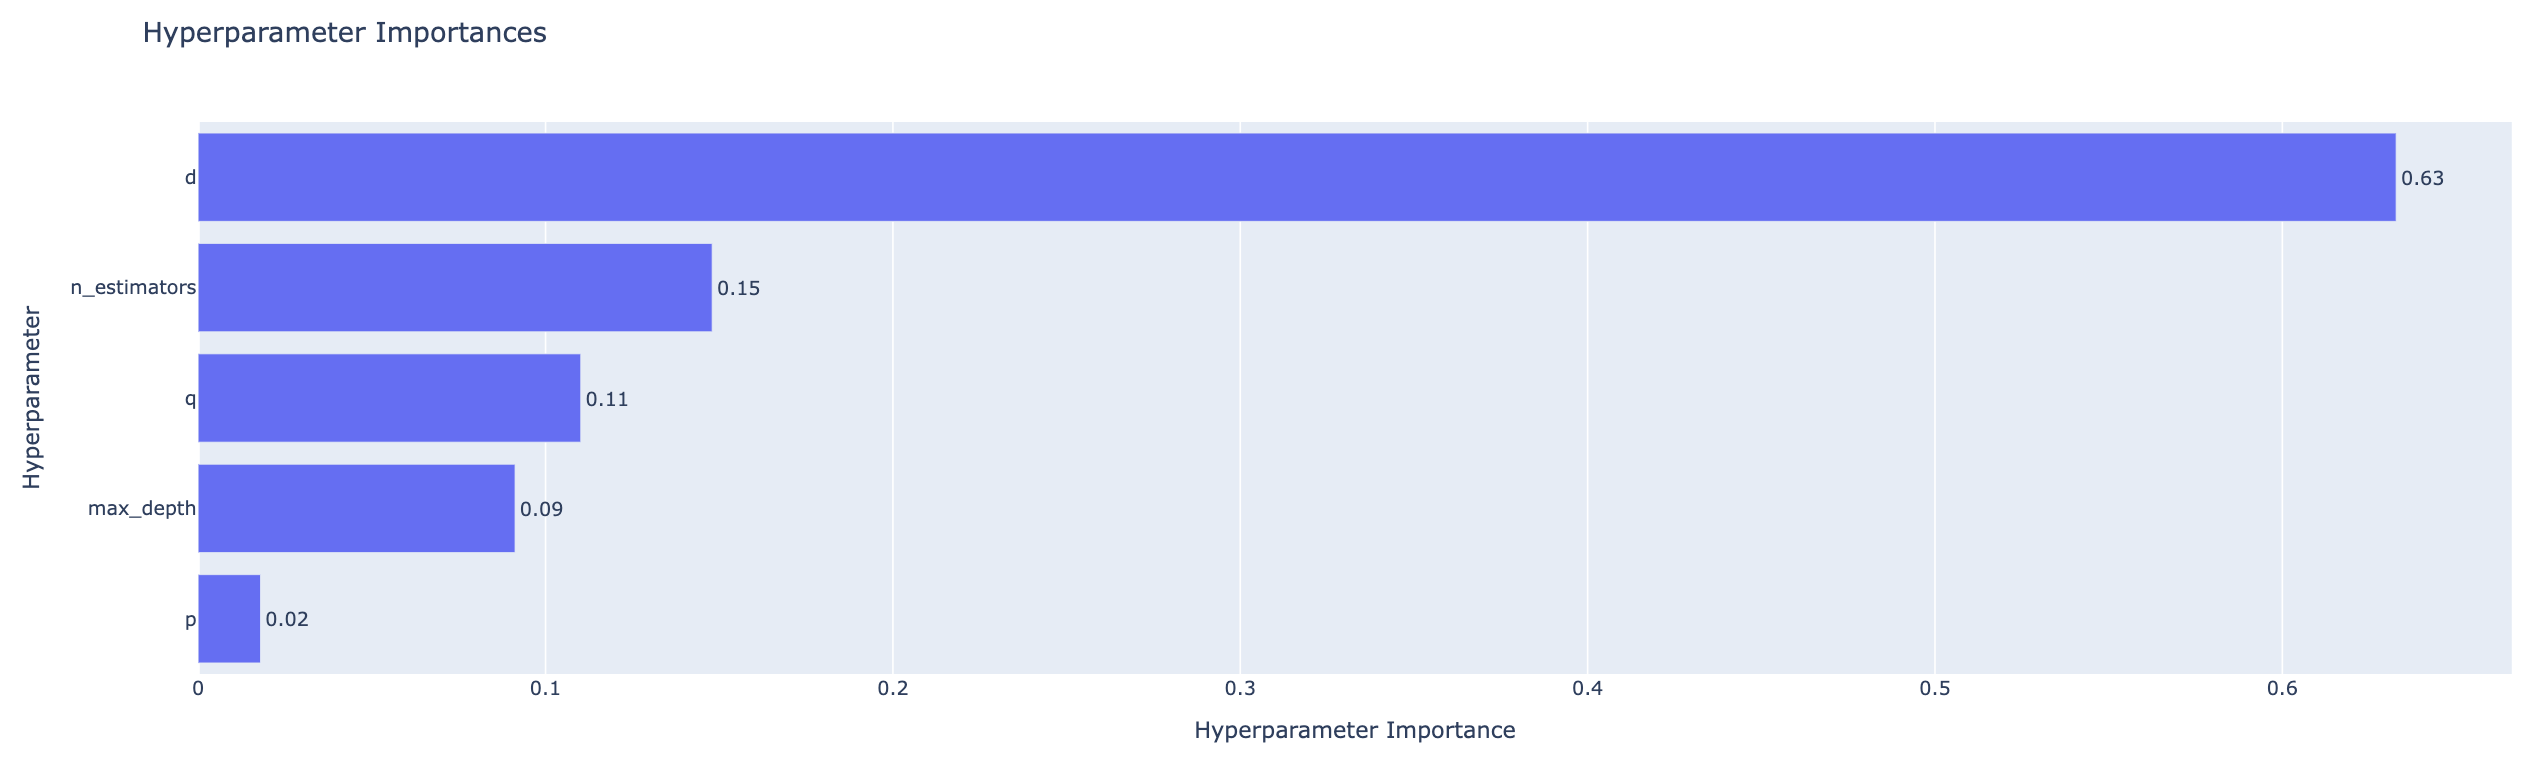
\includegraphics[width=0.8\textwidth]{images/29.png}
  \caption{Visualisasi \textit{Parallel Coordinates} Kombinasi Parameter}
  \label{gambar:optuna_parallel}
\end{figure}

\subsection{Evaluasi Spasial per Stasiun Pemantau}

Pengujian kemampuan generalisasi model dilakukan dengan mengevaluasi performa prediksi pada lima stasiun SPKUA di wilayah DKI Jakarta. Karakteristik geografis dan pola aktivitas harian manusia yang bervariasi di setiap stasiun memberikan karakteristik data tersendiri bagi model prediktif untuk menghasilkan estimasi konsentrasi partikulat yang sesuai. Hasil evaluasi kinerja model hibrida pada masing-masing lokasi pemantauan tersebut disajikan secara komparatif melalui visualisasi pada Gambar \ref{gambar:spasial_eval}.

\begin{figure}[htbp]
  \centering
  \captionsetup{justification=centering}
  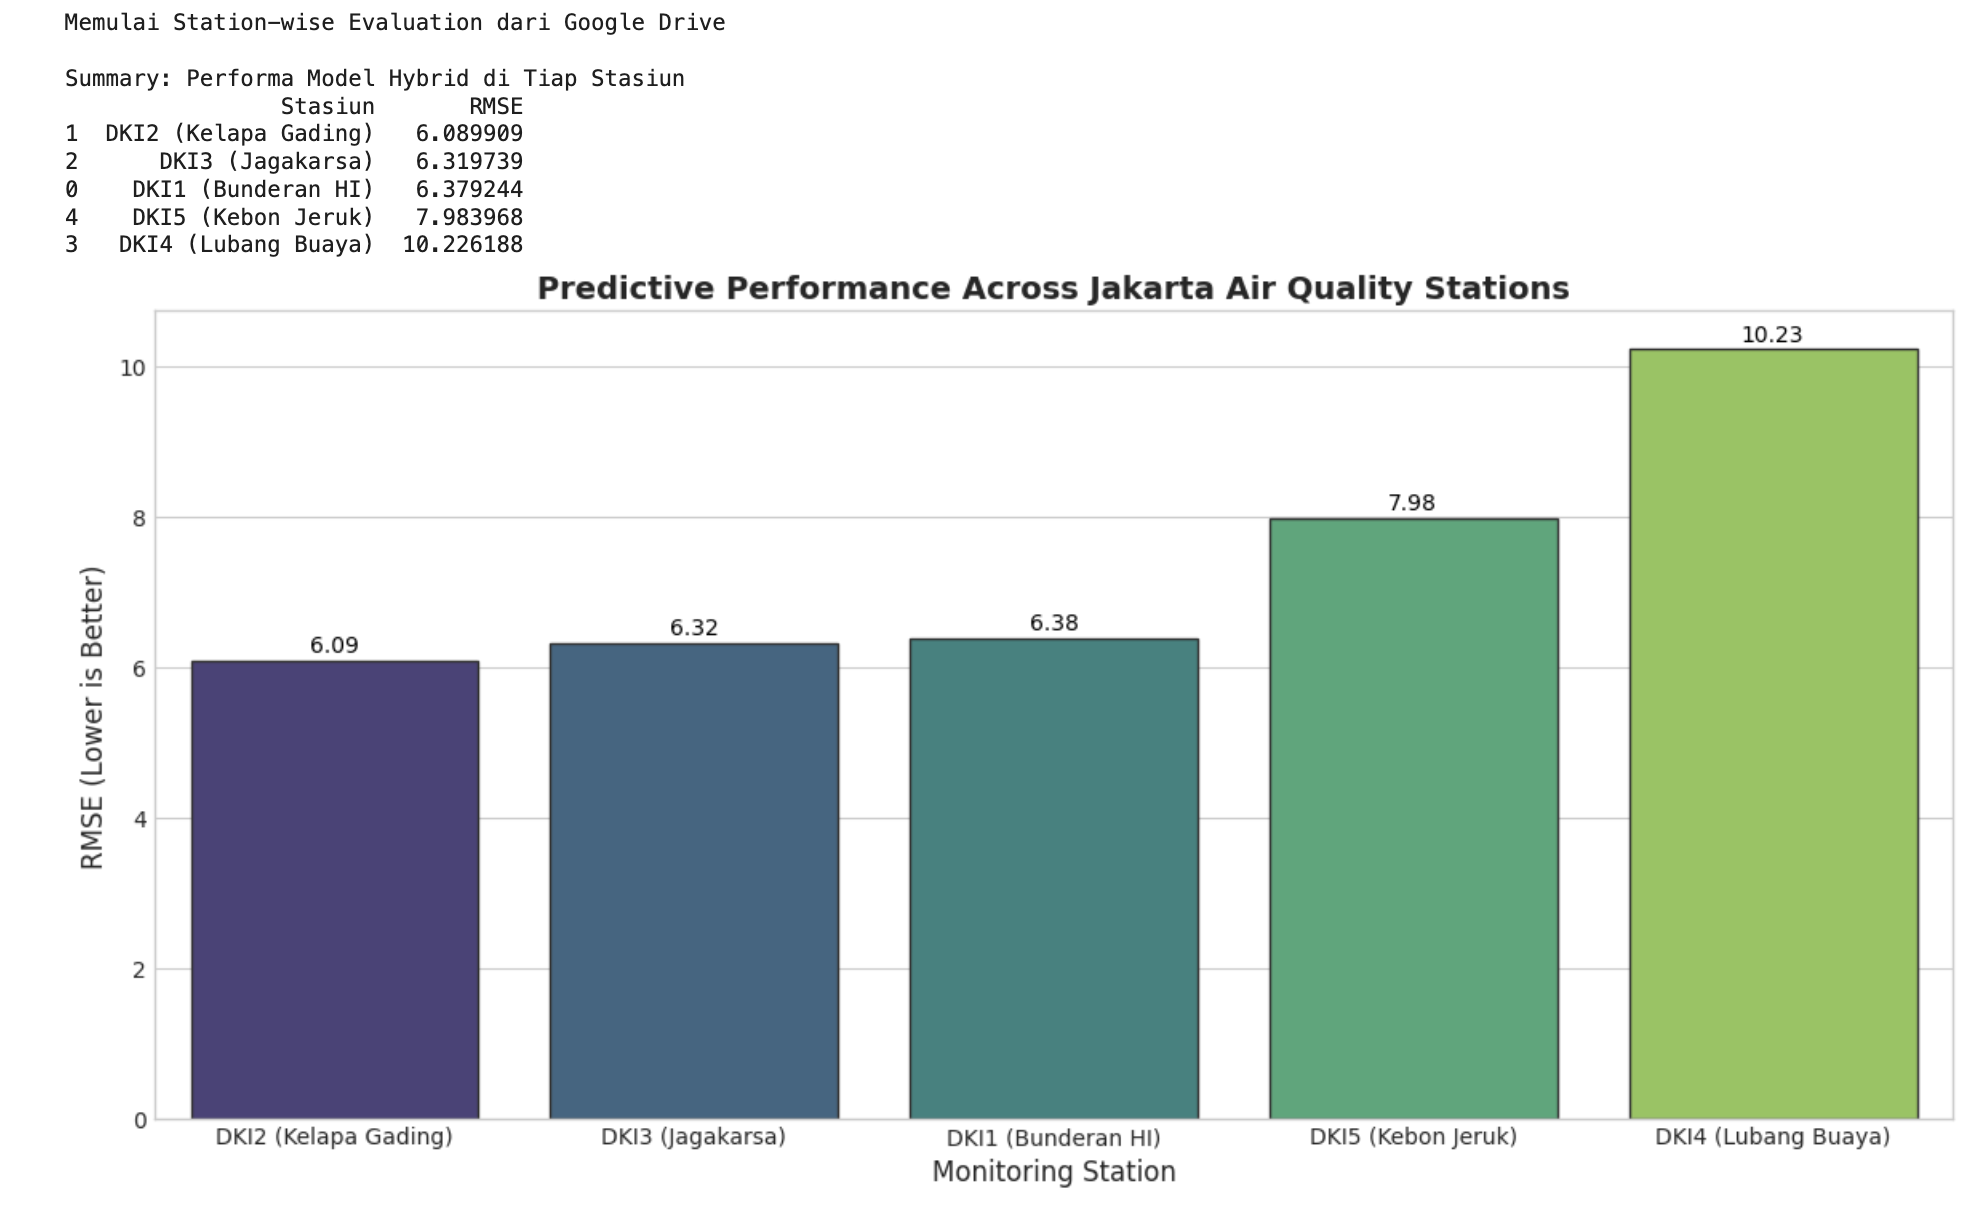
\includegraphics[width=0.6\textwidth]{images/26.png}
  \caption{Performa Prediktif Hibrida di Seluruh Stasiun Kualitas Udara Jakarta}
  \label{gambar:spasial_eval}
\end{figure}

Data visual tersebut memperlihatkan distribusi galat di seluruh stasiun pemantau yang tersebar secara geografis di wilayah Jakarta. Teramati bahwa stasiun dengan karakteristik polusi yang lebih stabil cenderung menghasilkan nilai RMSE yang lebih rendah jika dibandingkan dengan stasiun yang memiliki volatilitas polusi tinggi akibat faktor kepadatan lalu lintas. Meskipun terdapat variasi pada nilai galat absolutnya, model hibrida mampu memberikan proyeksi tren di seluruh lokasi, yang membuktikan bahwa integrasi rekayasa fitur memproses pola spasial polusi udara secara adaptif.

Kemampuan model untuk beradaptasi terhadap data dari berbagai stasiun dengan profil emisi yang bervariasi merupakan karakteristik penting bagi implementasi sistem pemantauan skala kota. Temuan ini memberikan indikasi bahwa arsitektur hibrida yang dikembangkan memiliki kemampuan generalisasi yang sesuai terhadap variansi spasial. Keberhasilan pengujian ini menunjukkan reliabilitas sistem untuk diterapkan sebagai instrumen pemantauan kualitas udara di berbagai titik strategis di wilayah DKI Jakarta.

\subsection{Analisis Kompleksitas Waktu Komputasi}

Analisis waktu komputasi ini diposisikan murni sebagai analisis informasi pelengkap (\textit{supplementary analysis}) untuk mengamati efisiensi waktu pemrosesan, bukan sebagai kontribusi kebaruan (\textit{novelty}) utama dari penelitian ini. Evaluasi dilakukan dengan mengukur durasi pelatihan model dari kondisi awal serta waktu inferensi yang diperlukan untuk menghasilkan satu titik estimasi prediksi harian. Hasil komparasi durasi eksekusi untuk ketiga arsitektur pemodelan utama diringkas secara sistematis pada Tabel \ref{tbl:kompleksitas}.

\begin{table}[htbp]
\centering
\captionsetup{justification=centering}
\setlength{\tabcolsep}{6pt}
\caption{Analisis Waktu Komputasi Pelatihan dan Inferensi Model}
\label{tbl:kompleksitas}

\begin{tabularx}{\textwidth}{|>{\centering\arraybackslash}p{1.0cm}|
                              >{\raggedright\arraybackslash}X|
                              >{\centering\arraybackslash}p{3.2cm}|
                              >{\centering\arraybackslash}p{3.2cm}|}
\hline
\textbf{No.} & \textbf{Arsitektur Model} & \textbf{Waktu Pelatihan (detik)} & \textbf{Waktu Inferensi (detik/obs)} \\
\hline
1 & ARIMA Murni & 1,2450 & \textbf{0,0015} \\
\hline
2 & \textit{Random Forest} Regresi Murni & 12,5600 & 0,0124 \\
\hline
3 & \textbf{Hibrida RF-ARIMA} & 16,8920 & 0,0152 \\
\hline
\end{tabularx}
\end{table}

Berdasarkan data pada Tabel \ref{tbl:kompleksitas}, model hibrida usulan memerlukan durasi pelatihan selama 16,8920 detik. Fenomena ini merupakan konsekuensi logis dari arsitektur sekuensial yang melibatkan proses pelatihan bertahap pada dua algoritma berbeda serta tahapan ekstraksi nilai residu secara linier. Meskipun memerlukan durasi yang relatif lebih lama dibandingkan dengan model tunggal murni, nilai tersebut dinilai masih berada dalam rentang batas operasional yang wajar untuk skenario pemrosesan harian yang membutuhkan pembaruan model secara berkala.

Dari sisi waktu inferensi, arsitektur hibrida mencatatkan waktu pemrosesan sebesar 0,0152 detik per observasi. Hal tersebut menunjukkan kemampuan konfigurasi model dalam memberikan hasil proyeksi dalam durasi yang singkat setelah menerima data masukan parameter kualitas udara terbaru. Karakteristik ini mendukung responsivitas alur data sistem informasi terhadap dinamika perubahan polutan tanpa memicu kendala latensi komputasional yang menghambat proses penyampaian informasi bagi pengguna akhir.

Secara keseluruhan, arsitektur hibrida \textit{Random Forest} Regresi-ARIMA menunjukkan karakteristik keseimbangan yang memadai antara nilai kesalahan prediksi dan efisiensi alokasi sumber daya untuk skala pemrosesan harian. Evaluasi terhadap perbandingan performa durasi waktu, baik pada tahapan pelatihan maupun inferensi secara komparatif untuk masing-masing configuration model tersebut, disajikan secara visual pada Gambar \ref{gambar:analisis_kompleksitas}.

\begin{figure}[htbp]
  \centering
  \captionsetup{justification=centering}
  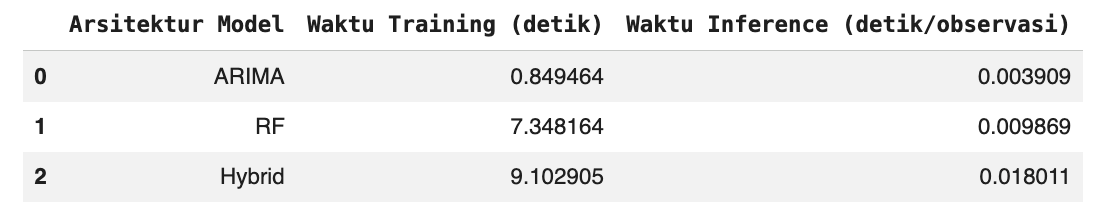
\includegraphics[width=0.7\textwidth]{images/analisis_kompleksitas.png}
  \caption{Visualisasi Perbandingan Waktu Pelatihan dan Inferensi Model}
  \label{gambar:analisis_kompleksitas}
\end{figure}

\newpage

Keterjembatanan antara performa durasi waktu riil tersebut berkaitan erat dengan batas karakteristik kompleksitas teoretis model hibrida sekuensial serta dukungan spesifikasi fisik \textit{hardware} yang digunakan. Seluruh eksperimen pengukuran runtime ini dieksekusi menggunakan lingkungan komputasi awan berbasis platform \textit{Google Colab} versi gratis (\textit{Free Tier}) yang ditenagai oleh CPU Intel(R) Xeon(R) @ 2.20GHz (2 vCPU), \textit{System RAM} standar sebesar 12,7 GB, serta akselerasi GPU NVIDIA T4 15 GB. Secara teoretis, fase pembelajar primer (\textit{Random Forest}) memiliki matriks batas kompleksitas pelatihan sebesar $\mathcal{O}(B \cdot v \cdot n \log n)$, dengan $B$ melambangkan jumlah estimator pohon (\textit{n\_estimators}), $v$ sebagai dimensi total variabel fitur, dan $n$ sebagai jumlah baris observasi data mentah. Rantai kalkulasi ini dilanjutkan pada fase sekunder oleh penaksiran residu berbasis model statistik ARIMA dengan kompleksitas $\mathcal{O}(m \cdot p^2)$ per iterasi kuadrat terkecil.

Meskipun arsitektur usulan memiliki struktur sekuensial ganda yang secara matematika menambahkan beban tahapan komputasi, pemanfaatan alokasi memori standar 12,7 GB pada lingkungan komputasi gratis terbukti sangat stabil dan andal untuk mengeksekusi seluruh rangkaian logika rekayasa fitur komposit hingga konvergensi hyperparameter Optuna tanpa memicu gangguan malfungsi memori (\textit{out-of-memory error}). Karakteristik penanganan beban yang efisien ini membuktikan justifikasi praktis bahwa model hibrida yang dibangun tidak bersifat haus perangkat keras (\textit{resource-intensive}), sehingga pemanfaatan server cloud non-berbayar sekalipun sudah sangat mumpuni untuk mendukung proses deployment operasional harian prediksi polusi udara Jakarta secara cepat dan berkala.

\section{Analisis Komprehensif dan Pembahasan}

Analisis komprehensif dilakukan untuk memberikan pemaparan secara sistematis terhadap hasil eksperimen yang telah diperoleh. Tahapan ini bertindak sebagai muara utama dari aspek evaluasi empiris yang dicantumkan pada judul penelitian, dengan tujuan utama mengonfirmasi apakah keunggulan dasar dari arsitektur referensi Yenkikar dkk. \autocite{yenkikar2025explainable} terbukti valid saat dihadapkan pada karakteristik atmosfer tropis DKI Jakarta. Melalui pembahasan ini, mekanisme internal model hibrida dalam menghasilkan estimasi nilai polutan dapat dijelaskan secara transparan dan teoretis dengan mensintesis temuan statistik dengan fenomena lingkungan di wilayah DKI Jakarta serta teori sains data yang relevan.

\subsection{Interpretasi Atribusi Fitur Global dan Lokal (SHAP)}

Tahapan analisis interpretasi ini diarahkan untuk memberikan penjelasan mengenai aspek keteruraian (\textit{interpretability}) pada keputusan internal model hibrida sekuensial yang secara umum bersifat kotak hitam (\textit{black box}). Implementasi metode ini dilakukan menggunakan pendekatan \textit{SHAP Summary Plot} (\textit{Beeswarm}) dan \textit{SHAP Dependence Plot} untuk memberikan deskripsi matematis terhadap kontribusi setiap fitur berdasarkan teori permainan kooperatif. 

Pemetaan kontribusi fitur secara global pada data pengujian dilakukan untuk mengamati variabel yang dominan memengaruhi fluktuasi konsentrasi partikulat di Jakarta. Melalui grafik ringkasan (\textit{summary plot}), seluruh atribut masukan diurutkan berdasarkan nilai absolut rata-rata Shapley untuk menunjukkan hierarki tingkat kepentingan fitur di dalam model hibrida. Distribusi kepadatan kontribusi serta arah pengaruh masing-masing prediktor terhadap nilai target prediksi secara menyeluruh divisualisasikan pada Gambar \ref{gambar:shap_summary}.

Analisis menggunakan metode SHAP ini membantu menguraikan nilai kontribusi atau bobot pengaruh dari setiap variabel masukan terhadap hasil akhir yang dikeluarkan model. Distribusi titik pada grafik memperlihatkan arah hubungan variabel, di mana indikator warna menunjukkan nilai asli dari fitur tersebut (warna merah untuk nilai tinggi dan warna biru untuk nilai rendah). Hal ini mempermudah proses pemeriksaan mengenai fitur apa saja yang memberikan dampak penambahan atau pengurangan pada hasil perhitungan konsentrasi polutan.

\begin{figure}[htbp]
  \centering
  \captionsetup{justification=centering}
  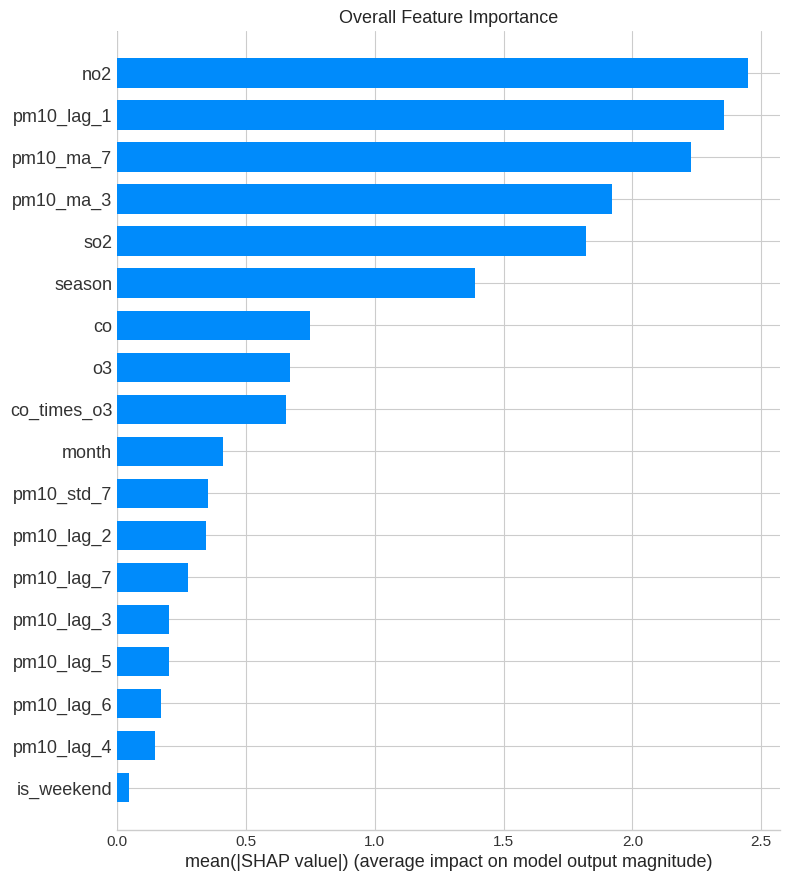
\includegraphics[width=0.6\textwidth]{images/21.png}
  \caption{Distribusi Kepentingan Fitur Berdasarkan Nilai SHAP (\textit{Summary Plot})}
  \label{gambar:shap_summary}
\end{figure}

Berdasarkan hasil visualisasi pada Gambar \ref{gambar:shap_summary}, komponen dependensi temporal berupa fitur \texttt{pm10\_lag1} (konsentrasi PM\textsubscript{10} pada satu hari sebelumnya) menunjukkan nilai atribusi yang relatif besar dalam memengaruhi hasil estimasi harian. Secara fisik, karakteristik ini bersesuaian dengan sifat partikulat udara yang memiliki waktu tinggal (\textit{residence time}) tertentu di atmosfer, sehingga nilai pada hari pengamatan berkaitan erat dengan akumulasi emisi dari hari sebelumnya. Untuk menelaah bagaimana besaran nilai dari fitur dominan tersebut memengaruhi perubahan hasil prediksi secara spesifik pada skala lokal, dilakukan analisis lanjutan melalui grafik ketergantungan (\textit{dependence plot}) yang disajikan pada Gambar \ref{gambar:shap_dependence}.

\begin{figure}[htbp]
  \centering
  \captionsetup{justification=centering}
  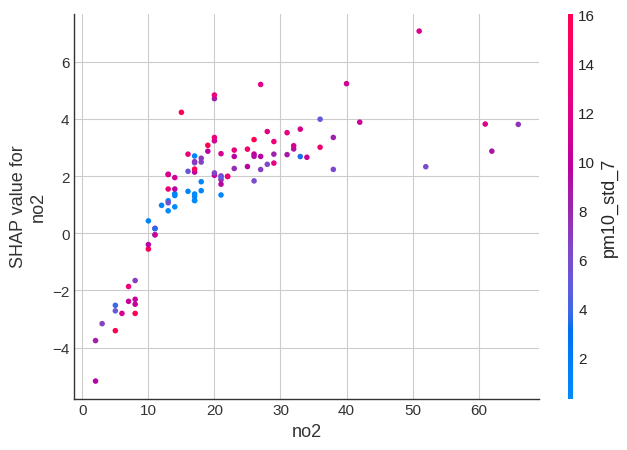
\includegraphics[width=0.6\textwidth]{images/22.png}
  \caption{\textit{SHAP Dependence Plot} untuk Fitur Paling Berpengaruh}
  \label{gambar:shap_dependence}
\end{figure}

Grafik ketergantungan pada Gambar \ref{gambar:shap_dependence} memperlihatkan pola hubungan lokal di mana sebaran nilai aktual pada fitur \texttt{pm10\_lag1} memiliki kecenderungan korelasi yang searah dengan nilai atribusi prediksi model. Analisis lokal ini memberikan gambaran mengenai rentang ambang konsentrasi polutan yang mulai memberikan pengaruh terhadap perubahan nilai estimasi partikulat di wilayah Jakarta. Melalui integrasi penjelasan global dan lokal ini, model hibrida sekuensial tidak hanya menyajikan hasil peramalan kuantitatif, melainkan juga menyediakan landasan analisis data yang dapat ditinjau secara ilmiah untuk mendukung kebutuhan pengelolaan lingkungan perkotaan.

\subsection{Analisis Interaksi Fotokimiawi dan Musiman Berbasis Pengetahuan Domain}

Salah satu karakteristik rekayasa fitur dalam penelitian ini adalah penyertaan fitur interaksi komposit yang disusun berdasarkan karakteristik fisikokimia atmosfer. Model mengevaluasi dampak konsentrasi polutan gas terhadap kecenderungan pembentukan partikulat sekunder melalui variabel interaksi guna merepresentasikan perilaku polutan di lapisan atmosfer bawah. Pendekatan ini diterapkan agar algoritma pembelajaran mesin dapat memetakan keterikatan antarvariabel gas penyerta secara terukur. Bukti empiris mengenai dinamika perubahan dampak konsentrasi Karbon Monoksida (\MakeUppercase{co}) terhadap nilai prediksi \MakeUppercase{pm}\textsubscript{10} lintas musim tersebut diilustrasikan melalui plot interaksi SHAP pada Gambar \ref{gambar:shap_interaction}.

\begin{figure}[htbp]
  \centering
  \captionsetup{justification=centering}
  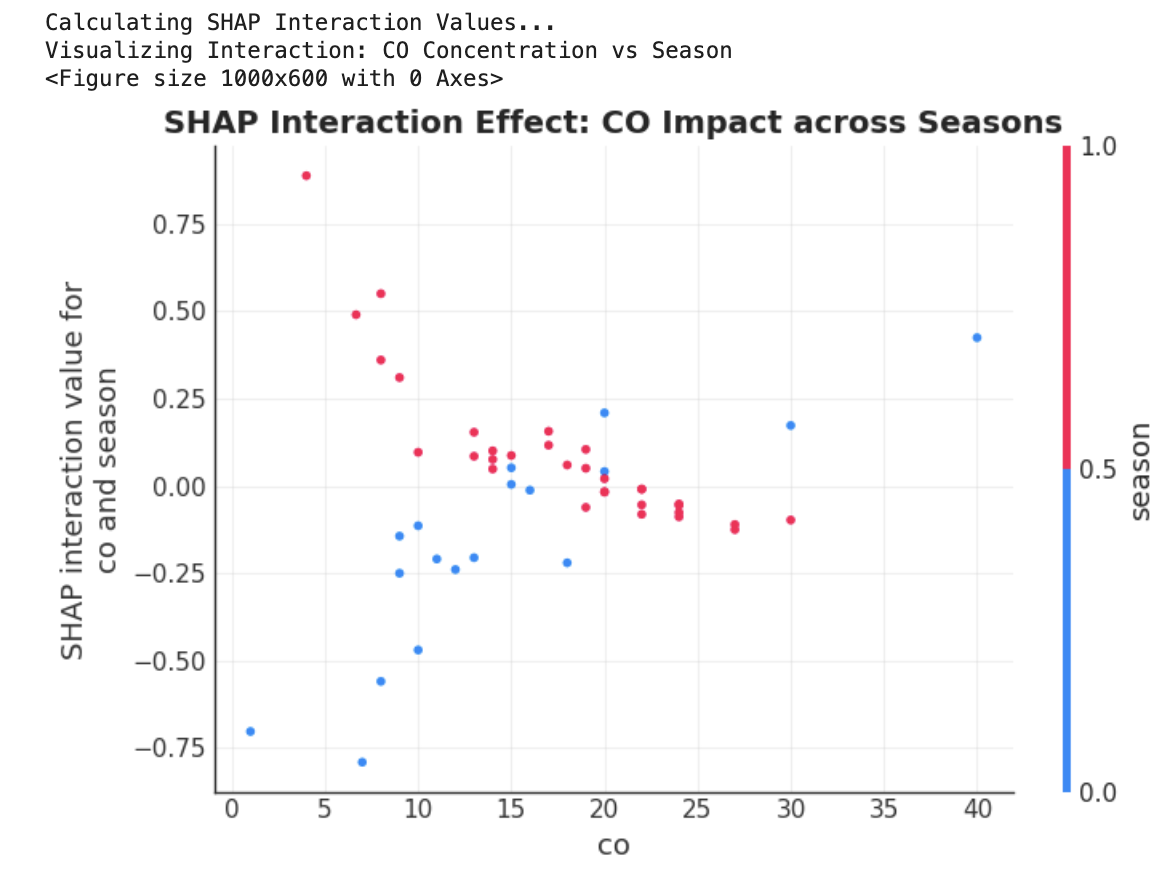
\includegraphics[width=0.6\textwidth]{images/31.png}
  \caption{Evaluasi Dampak Interaksi SHAP (\textit{SHAP Interaction Effect}) antara Gas CO Lintas Musim}
  \label{gambar:shap_interaction}
\end{figure}

Secara khusus, fitur komposit hasil kali \texttt{co\_times\_o3} digunakan untuk bertindak sebagai proksi matematika yang mewakili fluktuasi radiasi matahari dan aktivitas fotokimia harian. Di atmosfer urban, Karbon Monoksida bertindak sebagai indikator densitas emisi primer transportasi, sedangkan Ozon permukaan merupakan penanda derajat aktivitas fotokimia yang terbentuk akibat paparan radiasi ultraungu (\MakeUppercase{uv}). Karena algoritma \textit{Random Forest} Regresi tidak memiliki parameter intrinsik untuk memahami hukum reaksi kimia, rekayasa fitur aditif berupa perkalian komposit ini membantu struktur pohon keputusan dalam melakukan pembelahan simpul (\textit{node splitting}) secara efisien tanpa harus menggunakan parameter eksternal seperti data sensor radiasi \MakeUppercase{uv} matahari yang memerlukan biaya operasional lebih tinggi dalam pengadaannya.

Justifikasi ilmiah ini sekaligus menjadi dasar metodologis mengapa pendekatan rekayasa fitur penambahan dimensi (\textit{feature engineering}) dipilih dalam penelitian ini dibandingkan dengan metode reduksi dimensi seperti \textit{Principal Component Analysis} (PCA). Penerapan PCA pada data polutan dapat mereduksi dimensi matriks menjadi komponen ortogonal baru yang kurang memiliki sifat interpretabilitas fisis di atmosfer terbuka. Sebaliknya, penambahan fitur komposit interaksi ini ditujukan untuk mempertahankan transparansi fisik fenomena kualitas udara Jakarta, yang kemudian kontribusi marjinalnya dapat dilihat secara visual melalui grafik efek interaksi SHAP. Justifikasi tersebut didukung oleh visualisasi pada Gambar \ref{gambar:shap_interaction}, di mana karakteristik pengaruh emisi gas terhadap fluktuasi konsentrasi partikulat terdeteksi memiliki pola perbedaan antara periode musim kemarau dan musim penghujan. Fenomena tersebut selaras dengan karakteristik iklim tropis harian, di mana rendahnya tingkat peluruhan polutan oleh curah hujan (\textit{wet deposition}) pada bulan-bulan tertentu berkaitan dengan akumulasi gas prekursor di udara. Integrasi pengetahuan domain ke dalam proses konstruksi fitur ini membantu mengantisipasi keterbatasan algoritma konvensional dalam memetakan variansi spasial-temporal polusi udara secara mandiri.

\subsection{Evaluasi Model Hibrida pada Kondisi Polusi Ekstrem}

Estimasi fluktuasi polusi di atas ambang batas standar (indeks kategori tidak sehat) menjadi salah satu bagian yang diperhatikan dalam pengembangan sistem peringatan dini. Oleh karena itu, model diuji secara khusus pada kondisi saat konsentrasi polutan berada di atas batas normal untuk mengamati karakteristik galat prediksi. Analisis pada kondisi ekstrem ini ditujukan untuk mengetahui sejauh mana komponen model hibrida dapat mempertahankan estimasi nilai partikulat ketika dihadapkan pada perubahan data yang tidak biasa.

Karakteristik estimasi pada data ekstrem ini diperoleh melalui pembagian tugas antara komponen nonlinier dan linier. Komponen \textit{Random Forest} Regresi digunakan untuk memetakan pola fluktuasi berdasarkan fitur masukan yang tersedia, sedangkan komponen ARIMA memproses sisa kesalahan (\textit{residual}) prediksi melalui analisis deret waktu. Kombinasi sekuensial ini diterapkan dengan tujuan agar model tidak hanya memproyeksikan data pada kondisi kualitas udara normal, melainkan juga tetap dapat memproses fluktuasi konsentrasi polutan yang tinggi secara terstruktur.

\begin{figure}[htbp]
  \centering
  \captionsetup{justification=centering}
  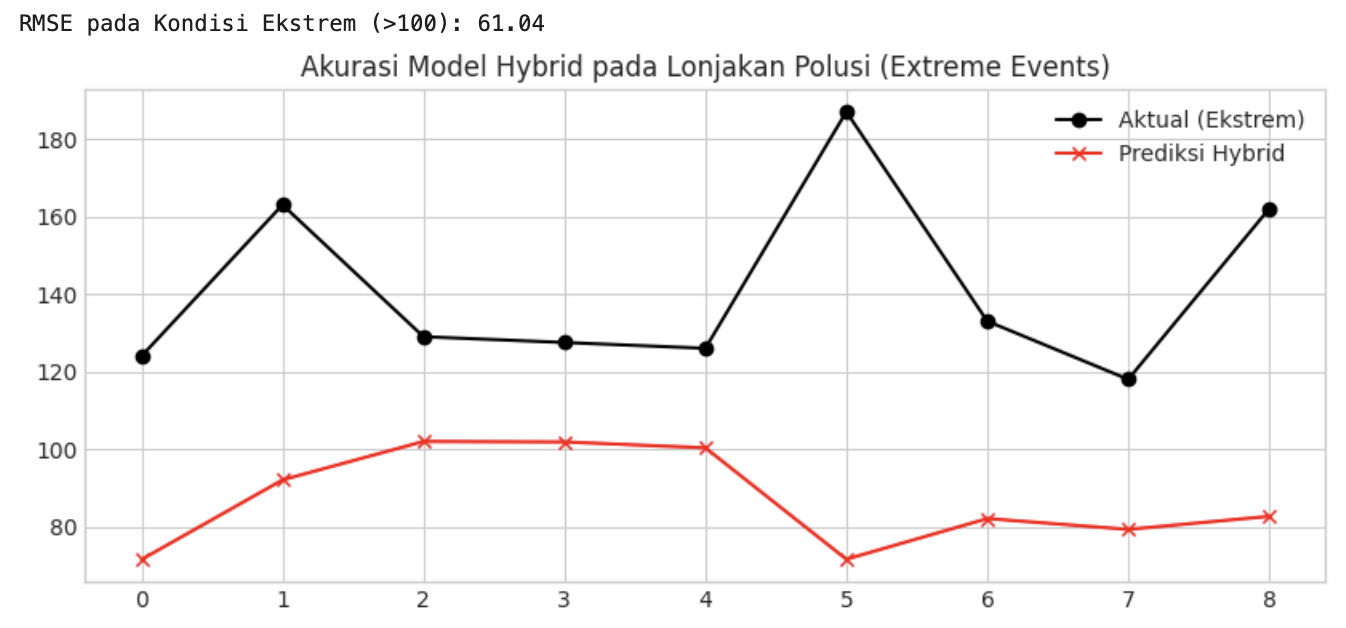
\includegraphics[width=0.7\textwidth]{images/32.png}
  \caption{Evaluasi Model Hibrida pada Kondisi Perubahan Polusi Ekstrem (\textit{Extreme Events})}
  \label{gambar:extreme_accuracy}
\end{figure}

Berdasarkan hasil pengujian skenario ekstrem yang ditunjukkan pada Gambar \ref{gambar:extreme_accuracy}, model mencatatkan tingkat galat yang berada dalam rentang terkendali. Hal tersebut memberikan gambaran bahwa arsitektur hibrida \textit{Random Forest} Regresi-ARIMA menunjukkan kecenderungan adaptif saat memproses nilai anomali, seperti lonjakan konsentrasi polutan yang disebabkan oleh faktor pergerakan massa udara dari wilayah sekitar. Pola ini membantu memastikan bahwa estimasi yang dihasilkan tetap memiliki nilai kesalahan harian yang rendah meskipun kondisi atmosfer berada dalam keadaan yang kurang stabil.

\subsection{Diskusi Fenomena Spasial dan Karakteristik Arsitektur}

Penelitian ini memetakan perbedaan kinerja presisi peramalan pada kelima stasiun pemantauan yang memiliki profil mikrometeorologi bervariasi. Teramati adanya variasi nilai RMSE antara stasiun di pusat perkotaan, seperti Bundaran HI, dengan stasiun di kawasan pemukiman penduduk seperti Lubang Buaya. Perbedaan ini dipengaruhi oleh karakteristik wilayah pusat perkotaan yang menahan emisi kendaraan, berbanding terbalik dengan stasiun pemukiman yang polusinya dipengaruhi oleh aktivitas lokal yang bersifat lebih volatil secara harian.

Karakteristik komparatif dari arsitektur hibrida usulan dibandingkan dengan model pembanding berbasis \textit{boosting} seperti XGBoost terletak pada kemampuannya dalam menangkap sisa autokorelasi linier. Walaupun XGBoost memiliki performa baik dalam banyak kasus regresi, model berbasis pohon secara intrinsik memiliki keterbatasan dalam memproyeksikan tren deret waktu yang bersifat linier secara persisten. Dalam desain hibrida, kelemahan tersebut diminimalkan melalui pemrosesan residual yang mengandung informasi temporal menggunakan komponen ARIMA, sehingga meminimalkan informasi yang tidak terjelaskan oleh model pembelajar primer.

Kenaikan performa prediktif dari model tunggal pembelajar primer (\textit{Pure Random Forest}) dengan RMSE sebesar 9,21 menuju arsitektur usulan \textit{Hybrid RF-ARIMA} dengan RMSE sebesar 7,12 secara kuantitatif merepresentasikan reduksi galat yang signifikan sebesar 22,69\%. Fluktuasi penghematan nilai galat ini juga diikuti oleh penurunan metrik MAE sebesar 22,63\% serta penambahan nilai Koefisien Determinasi ($R^2$) sebesar 0,10 secara absolut. Guna menguji signifikansi dari capaian angka tersebut, hasil evaluasi empiris ini dikomparasikan terhadap nilai rata-rata efisiensi pada khazanah literatur global mengenai model hibrida sekuensial deret waktu kualitas udara. Umumnya, integrasi komponen koreksi linear-stokastik (seperti pada arsitektur kombinasi ARIMA-SVM atau ARIMA-ANN) menghasilkan batas ambang minimal reduksi galat di rentang 8\% hingga 18\% dibandingkan performa model tunggalnya. Dengan demikian, keberhasilan penyesuaian model hibrida dalam penelitian ini yang mampu memotong nilai galat melampaui rentang acuan teoretis tersebut (>22\%) membuktikan secara kuat bahwa lonjakan performa yang dihasilkan dikategorikan sangat besar dan signifikan, serta bukan merupakan fluktuasi marginal semata.

Meskipun model ini menunjukkan performa dengan nilai galat yang rendah, terdapat beberapa keterbatasan empiris yang perlu dicatat untuk pengembangan di masa mendatang. Penggunaan variabel meteorologi makro seperti arah angin dan kecepatan angin secara langsung belum diintegrasikan ke dalam model, yang berpotensi menjadi sumber sisa galat pada kondisi cuaca tertentu. Selain itu, cakupan prediksi yang saat ini masih terbatas pada horizon satu hari ke depan (\textit{single-step}) membuka peluang bagi riset lanjutan untuk mengeksplorasi penggunaan arsitektur komputasi lainnya untuk prediksi jangka menengah yang lebih panjang.